\section{Experiments}


In this section, we evaluate the performance of our method qualitatively and quantitatively.
First, we introduce the used datasets.  
Then we compare our method with the state-of-the-art human relighting method Relighting4D \cite{Relighting4D}.
Since our geometry reconstruction is improved by the proposed invertible deformation field, we also compare our method with the state-of-the-art video-based human geometry reconstruction methods ARAH \cite{ARAH} and \citet{peng2022animatable}.
Next, we perform ablation studies to validate our key design choices.
Finally, we show the synthesized results on various characters with various body motions under various lightings, and video results can be seen in the supplemental video.

\subsection{Datasets}

We use both real and synthetic datasets for comparisons and evaluations.
For the real dataset, we use multi-view dynamic human datasets including the ZJU-MoCap \cite{neuralbody}, Human3.6M \cite{h36m}, DeepCap \cite{deepcap} and PeopleSnapshot \cite{alldieck2018video} dataset.
To perform a quantitative evaluation, we create a new synthetic dataset.
We leverage 4 rigged characters from Mixamo\footnote{\url{https://www.mixamo.com/}} and transfer the body motion from the ZJU-MoCap dataset to generate motion sequences. Each sequence contains 100 frames.
Then, we use Blender\footnote{\url{https://www.blender.org/}} to render multi-view videos under different illuminations with HDRI environment maps from PolyHaven\footnote{\url{https://polyhaven.com/}}.
Besides, we use 4 OLAT light sources for relighting evaluations.

\subsection{Comparisons}
Since Relighting4D \cite{Relighting4D} is the state-of-the-art for video-based human motion relighting, we compare our full method with it on albedo estimation, lighting reconstruction, and relighting under training/novel poses.
Body geometry is an intermediate result of our method, we also compare it with the state-of-the-art video-based human geometry reconstruction methods \citet{peng2022animatable} and ARAH \cite{ARAH}.

\textbf{Material Estimation and Relighting.}
The comparison results with Relighting4D \cite{Relighting4D} are shown in Fig.\ref{fig:albedo_rec}.
Relighting4D cannot disentangle the lighting and appearance very well, as we can see noticeable errors on both the estimated environment map and the reconstructed albedo.
For example, there are shadows wrongly baked into albedo in the result on the top right side.
Besides, some lighting information is backed into albedo in the result on the bottom right side.
For numerical comparisons, we use Peak Signal-to-Noise Ratio (PSNR), Structural Similarity Index Measure (SSIM) \cite{ssim}, and Learned Perceptual Image Patch Similarity (LPIPS) \cite{lpips} as metrics.
In Tab.\ref{tab:syn}, we show the numerical albedo estimation result on synthetic data, which also indicates our improvement in albedo estimation.
Tab.\ref{tab:syn} also shows the final relighting results for both training poses and novel poses, both show that we achieve noticeably better results than Relighitng4D.
Note that for novel poses, there are misalignments in the geometry between the animated geometry and the ground truth geometry, which leads to noticeable performance drops for novel poses.
Besides, qualitative results for relighting on real datasets are shown in Fig.\ref{fig:relit_real} (please zoom in for better comparison).
The overall lighting effect is better rendered by our method as shown on the left, and the spatial variant effect caused by point light is also correctly generated by our method as shown on the right due to the success of visibility modeling. More video results can be seen in our supplementary video.
Notice that as Relighting4D relies on per-frame latent codes to model the dynamics, it does not support novel poses synthesis by design. So, when performing relighting for a novel pose, we find the closest pose in its training poses and use its latent code for inference.

\textbf{Geometry Reconstruction.}
We evaluate different methods on our synthetic dataset with ground truth geometry and use point-to-surface distance (P2S) and Chamfer Distance (CD) as metrics.
The results as shown in Tab.\ref{tab:geo}, our method outperforms the compared two methods on all test sequences. 
We also show qualitative comparisons of rendering images in the real dataset in Fig.\ref{fig:geo_artifact}.
We can find that there are obvious artifacts in the results of \citet{peng2022animatable} and ARAH in the elbow and hand regions.
While the result of our method does not suffer from the artifacts, as our mesh-based inverse skinning helps to find accurate correspondences between the observation space and the canonical space.
In contrast, \citet{peng2022animatable} use posed SMPL models to compute the backward skinning weights which leads to worse correspondences, especially for regions with body contacts.
ARAH involves iterative root-finding to compute the correspondences, but the optimization sometimes fails to converge, thus also leading to artifacts.


\begin{table}[]
\begin{center}
\scalebox{0.85}{
\begin{tabular}{ccccccc}
\hline
                     & Method      & S1    & S2    & S3    & S4    & Avg \\ \hline
\multirow{5}{*}{P2S$\downarrow$} & Peng et al. & 0.387 & 0.359 & 0.339 & 0.339 & 0.356   \\
                     & ARAH        & 0.317 & 0.340 & 0.325 & 0.280 & 0.316   \\
                     & Ours w/o MIS  & 0.241 & 0.230 & 0.234 & 0.241 & 0.237   \\
                     & Ours w/o $\mathbf{W}$ & 0.246 & 0.247 & 0.243 & 0.256 & 0.248   \\
                     & Ours        & \textbf{0.185} & \textbf{0.179} & \textbf{0.182} & \textbf{0.184} & \textbf{0.182}   \\ \hline
\multirow{5}{*}{CD$\downarrow$}  & Peng et al. & 0.656 & 0.864 & 0.521 & 0.528 & 0.642   \\
                     & ARAH        & 0.531 & 0.714 & 0.477 & 0.441 & 0.541   \\
                     & Ours w/o MIS & 0.462 & 0.666 & 0.423 & 0.391 & 0.485   \\
                     & Ours w/o $\mathbf{W}$ & 0.479 & 0.700 & 0.427 & 0.424 & 0.507   \\
                     & Ours        & \textbf{0.395} & \textbf{0.609} & \textbf{0.358} & \textbf{0.363} & \textbf{0.431}   \\ 
\hline
\end{tabular}
}
\caption{Quantitative comparison of the reconstructed geometry on synthetic data.}
\label{tab:geo}
\end{center}
\end{table}


\subsection{Ablation Study}
\label{sec:ablation}
Here, we evaluate our two key components: mesh-based inverse skinning (MIS) and part-wise visibility estimation. 
The MIS based on the invertible deformation makes it possible to deform the more accurate mesh in the canonical space to the observation space to calculate skinning weights. 
Otherwise, the naked SMPL mesh with large geometry errors has to be used. 
So, we compare our method with using the SMPL mesh in weights calculation. 
Besides, using the part-wise design achieves accurate light visibility estimation, which is crucial to generate self-occlusion effects on bodies.
To evaluate it, we compare it with two alternatives, removing the light visibility module and using only one neural network to predict the light visibility.

\textbf{Mesh-based Inverse Skinning.}
As shown in Tab.\ref{tab:geo}, the reconstruction errors without the mesh-based inverse skinning are consistently larger.
We also show the qualitative result in Fig.\ref{fig:geo_artifact}, using SMPL mesh to compute the skinning weights leads to artifacts in the contact regions.

Besides, we evaluate the effect of the condition of skinning weights $\mathbf{W}$ (in Sec.~\ref{sec:geo_rec}) in the invertible deformation network.
As shown in Tab.\ref{tab:geo}, we can also find that removing the condition of $\mathbf{W}$ also leads to worse results.


\textbf{Part-wise Visibility Estimation.}
We show quantitative comparisons in Tab.\ref{tab:syn}, the results show that although the albedo map reconstruction qualities are similar, our method with part-wise visibility estimation achieves the best results on relighting.
Furthermore, We show qualitative results in Fig.\ref{fig:ablation_lvis}.
We can see that without light visibility modeling (results in the fourth column), the self-occlusion effect cannot be generated at all.
With the baseline light visibility modeling, self-occlusion can be partly generated for some poses (results of the third column).
For our final solution, the received lighting for different body regions on the novel poses are well modeled and thus the relighting results are consistent with the ground truth rendering.

\begin{figure}[t]
\begin{center}
   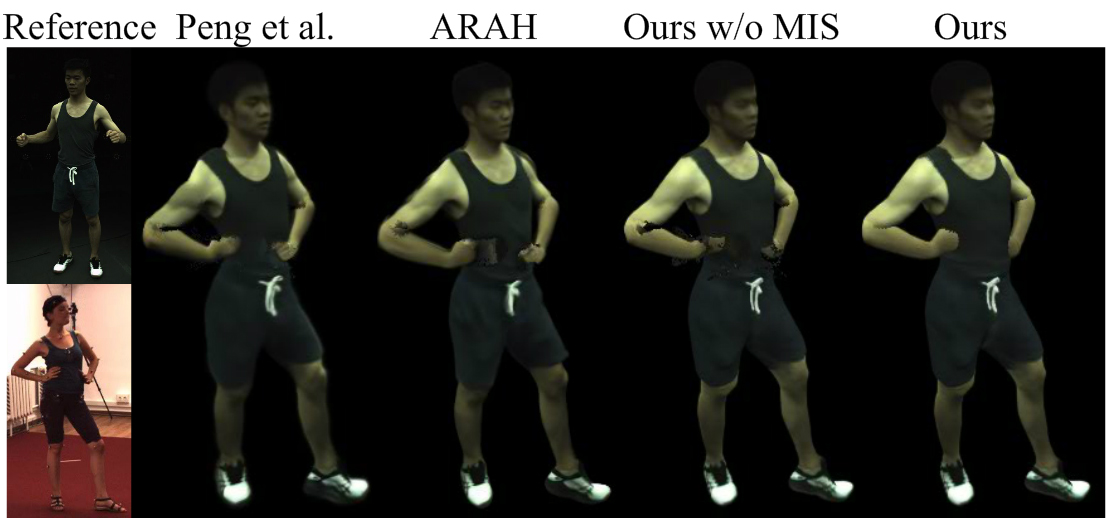
\includegraphics[width=1.0\linewidth]{./fig/geo_artifact.jpg}
\end{center}
\caption{Qualitative results of novel poses synthesis on real data. This novel pose results reflect the accuracy of the reconstructed geometry to a certain extent. }
\label{fig:geo_artifact}
\end{figure}

\begin{figure}[t]
\begin{center}
   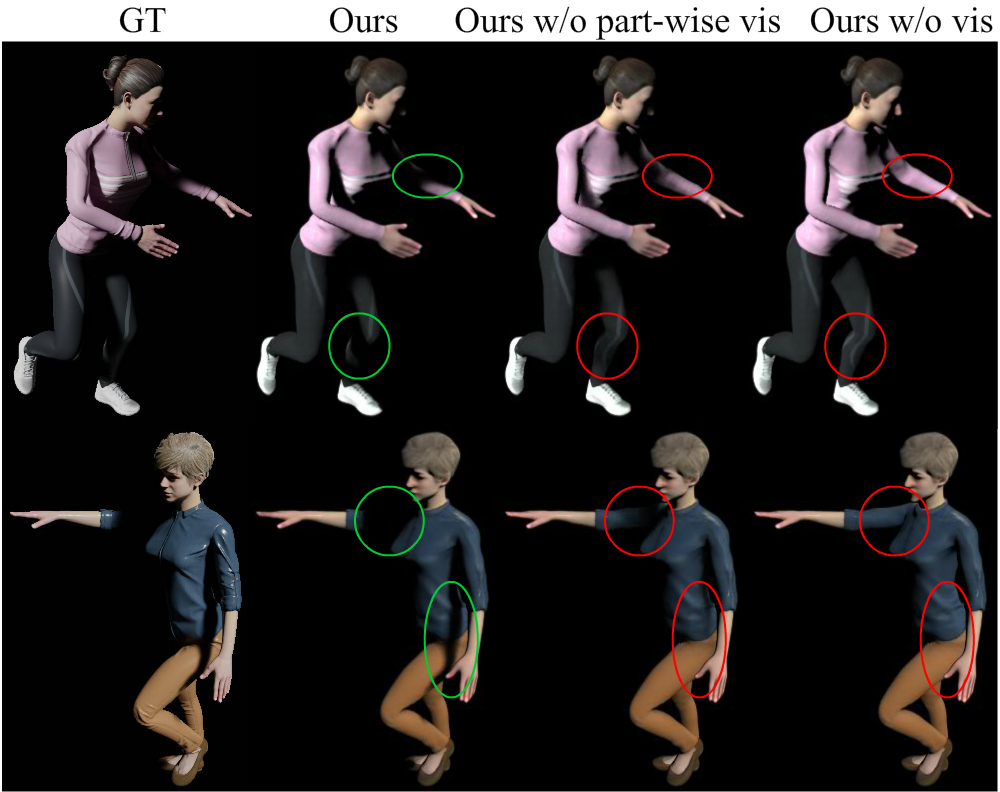
\includegraphics[width=1.0\linewidth]{./fig/ablation_lvis.jpg}
\end{center}
\caption{Ablation study on part-wise light visibility. See our method synthesizing plausible self-occlusions.}
\label{fig:ablation_lvis}
\end{figure}

